\section{Fit to invariant mass distribution of the $\Bs\to\Ds\hadron\pion\pion$ candidates}
\label{sec:Massfit}

Probability density functions (PDFs) are used to describe the signal and background components of the invariant mass distributions of $\Bs\Ds\pion\pion\pion$ and $\Bs\to\Ds\kaon\pion\pion$ candidates.
They are obtained from a mixture of data-driven approaches and simulation, where the simulated distributions are corrected for kinematic differences between the simulation and data.\newline
The shape of the signal candidates in the $\Bs\to\Ds\kaon\pion\pion$ and $\Bs\to\Ds\pion\pion\pion$ distributions are modelled using a Johnsons's SU function~\cite{10.2307/2332539}, 
which results from a variable transformation of a normal distribution to allow for asymmetric tails. 
It provides a good description of the Gaussian signal peak, as well as reconstruction effects and radiative tails of the distribution.
The shape of the Johnson's SU function is determined using simulation for both modes and subsequently fixed in the fit to data. 
To compensate small differences between the simulation and data, scale factors for the mean and width of the PDFs are introduced and floated during the fit.
For the functional form of the combinatorial background, second order polynomials are used whose parameters are determined, for each $\Ds$ mode separately, in the fit to data.
The partially reconstructed background component is described using an empirical description that is derived from simulation. 
In the fit to $\Bs\Ds\pion\pion\pion$ data, all parameters are fixed to the ones obtained from simulation, except for a width parameter to account for small discrepancies between data and simulated samples.
For the fit to $\Bs\Ds\kaon\pion\pion$ data, the shape is fixed to the one obtained from the control mode.
A small fraction of $\Bs\Ds\pion\pion\pion$ an $\Bs\Ds^{*}\pion\pion\pion$ decays, where one of the pions is misidentified as a kaon, contaminate the $\Bs\to\Ds\kaon\pion\pion$ data sample.
Simulated samples of the control mode is used to determine the shape of this background, where the mass hypothesis of one pion is changed to a kaon during the reconstruction process. 
The yield of this component is estimated from simulation and fixed in the fit to $\Bs\to\Ds\kaon\pion\pion$ data, 
taking into account the misidentification probability given the particle identification requirements imposed during the selection process.\newline
Figure \ref{fig:massFit} shows the result of the fit to the invariant mass distributions of $\Bs\to\Ds\pion\pion\pion$ and $\Bs\to\Ds\kaon\pion\pion$ candidates, 
where the data from Run I and II, as well as all $\Ds$ decay modes, are overlaid.  

\begin{figure}[h]
\centering
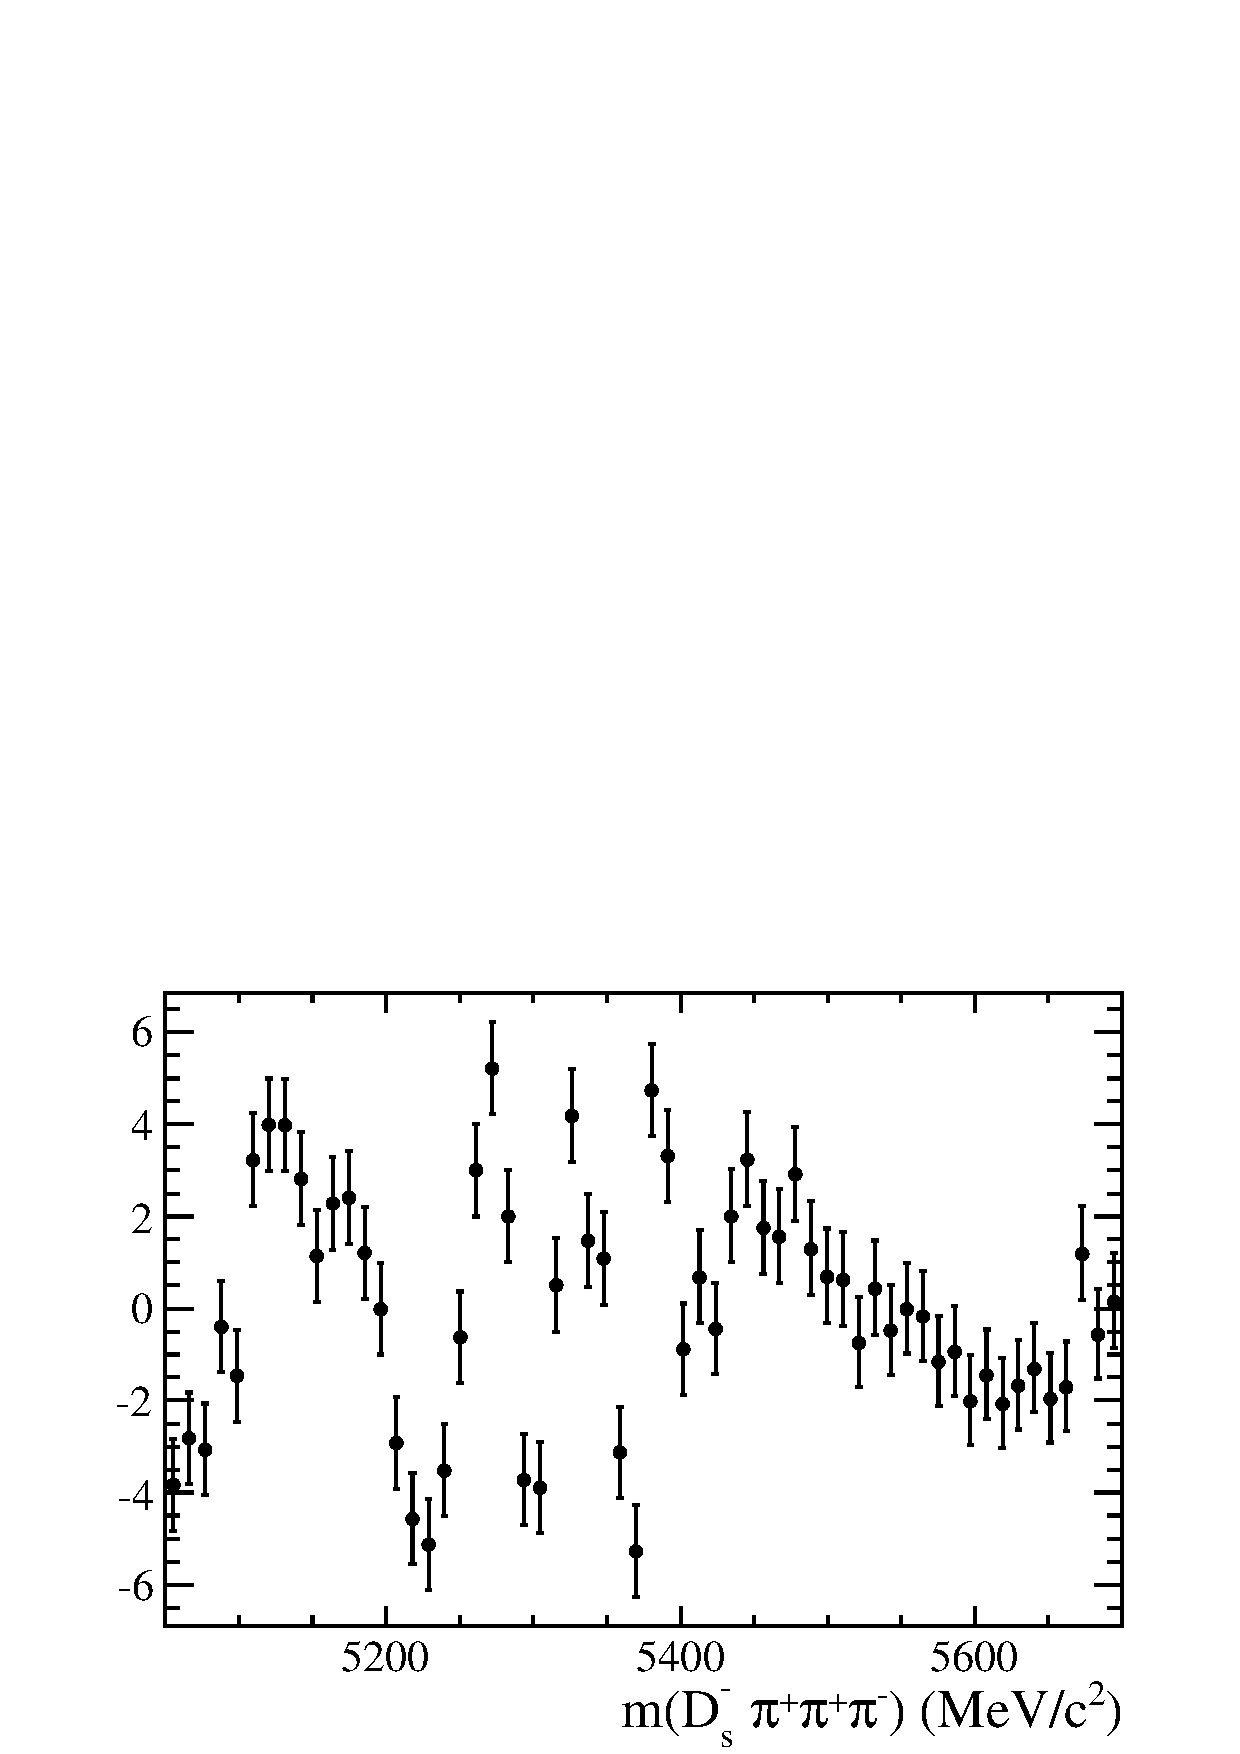
\includegraphics[height=!,width=0.49\textwidth]{figs/MassFit/norm_pull.pdf}
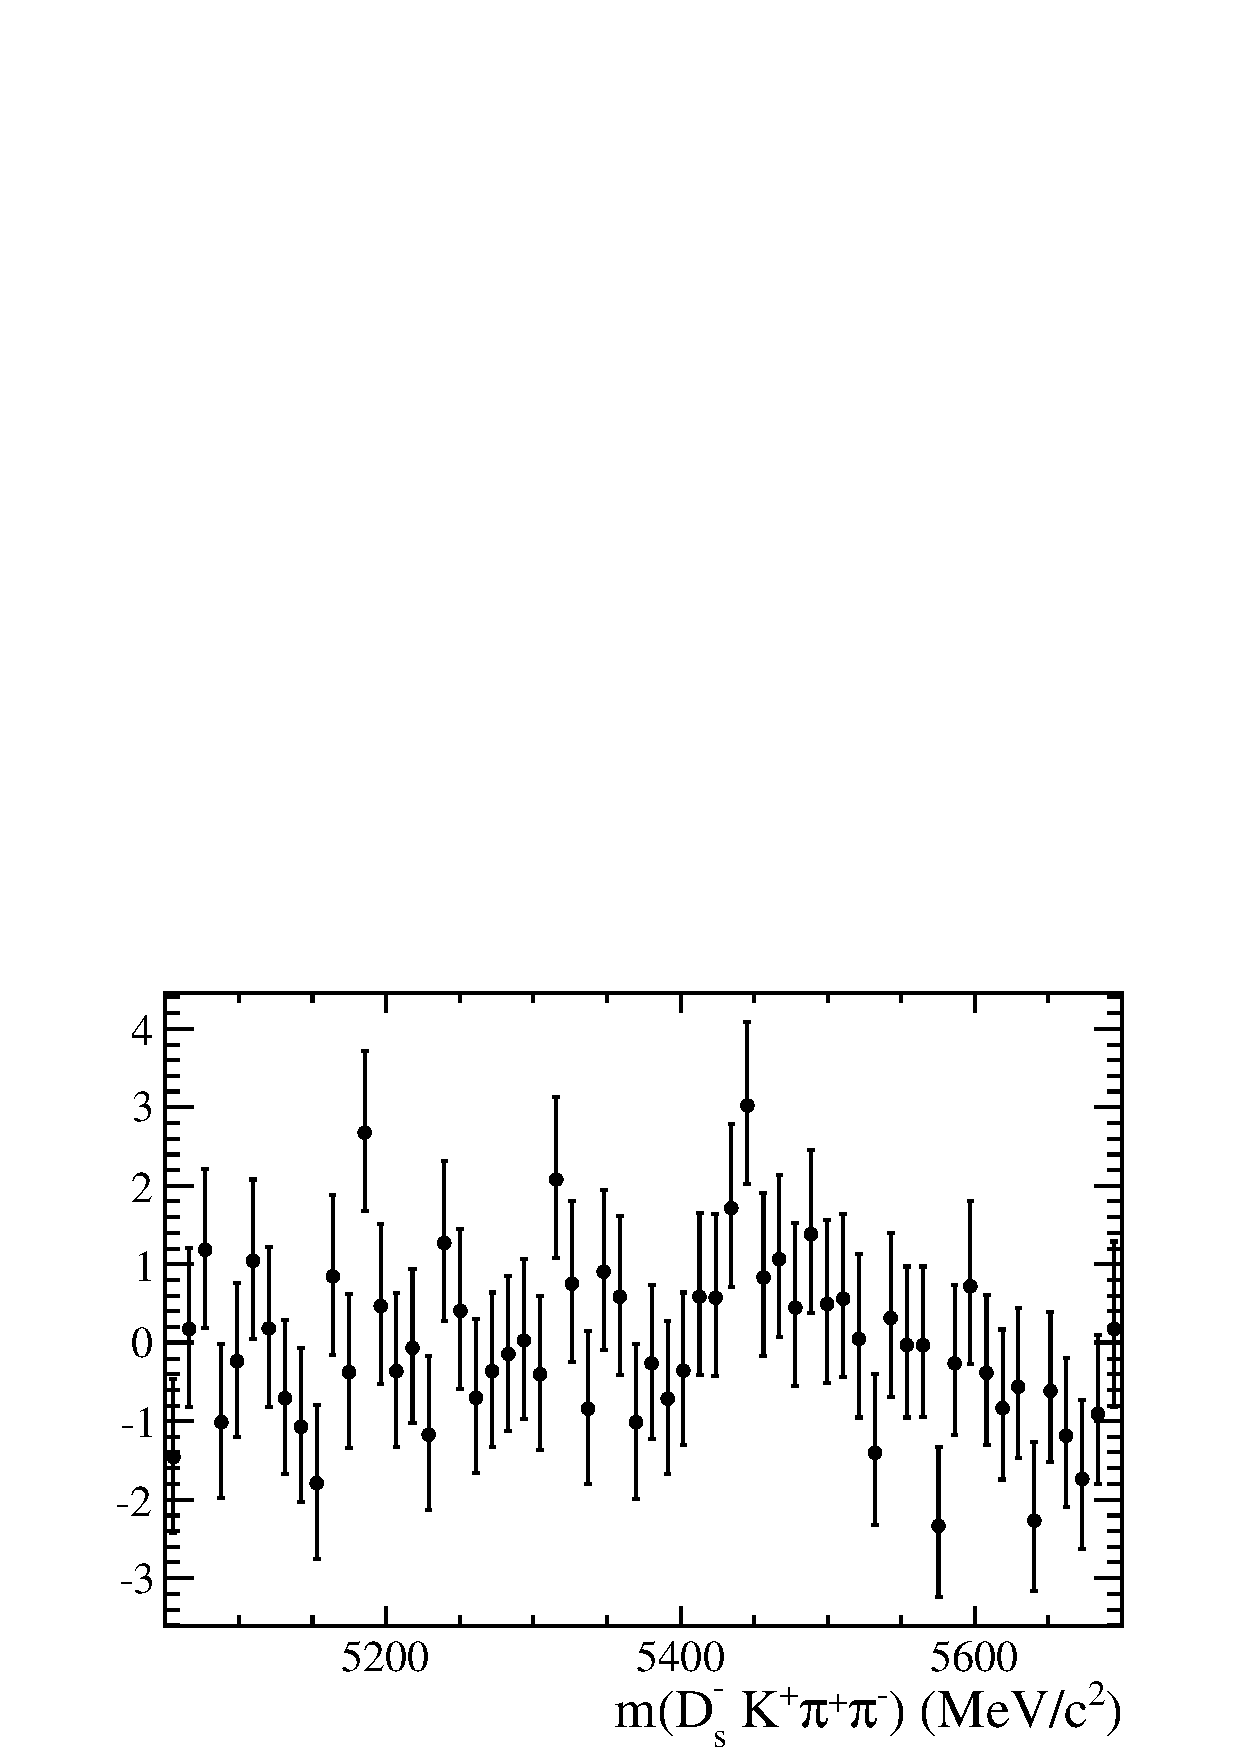
\includegraphics[height=!,width=0.49\textwidth]{figs/MassFit/signal_pull.pdf}
\caption{Invariant mass distribution of $\Bs\to\Ds\pion\pion\pion$ (left) and  $\Bs\to\Ds\kaon\pion\pion$ (right) candidates. The fit described in the text is overlaid.}
\label{fig:massFit}
\end{figure}
